\documentclass[letterpaper]{article} % DO NOT CHANGE THIS
\usepackage[submission]{aaai2027}  % double-blind submission format
\usepackage[hyphens]{url} % DO NOT CHANGE THIS
\usepackage{graphicx} % DO NOT CHANGE THIS
\urlstyle{rm} % DO NOT CHANGE THIS
\def\UrlFont{\rm}  % DO NOT CHANGE THIS
\usepackage{natbib}  % DO NOT CHANGE THIS AND DO NOT ADD ANY OPTIONS TO IT
\usepackage{caption} % DO NOT CHANGE THIS AND DO NOT ADD ANY OPTIONS TO IT
\frenchspacing  % DO NOT CHANGE THIS
\usepackage{amsmath}
\usepackage{amssymb}
\usepackage{booktabs}
\usepackage{array}
\pdfinfo{
/TemplateVersion (2027.1)
}
\setcounter{secnumdepth}{2} % section numbers for \S\ref

\graphicspath{{../out/figures/}}

\title{Democracy Bench: Can a Language Model Be Steered Toward the Public Without Eroding Democratic Rights?}

\author{
    Anonymous Submission
}
\affiliations{
    Paper submitted to the AAAI-27 Special Track on AI for Social Impact
}

\begin{document}
\maketitle

\begin{abstract}
Civil servants and public bodies are meant to track the opinions and preferences of
their constituents, and democracies have built mechanisms for exactly that: elections,
consultations, and opinion polls all filter the public's views into policy. It is far
less clear whose opinions and values the AI models now entering government reflect. We
introduce \textbf{Democracy Bench}, an evaluation harness that measures whether a
language model tracks public attitudes, across waves of the British Social Attitudes
survey, and whether those attitudes can then be instilled in it. Its central design is a
boundary between \emph{contestable} policy preferences (tax, public spending,
healthcare) and a \emph{rights floor} that must hold regardless (due process, the right
to appeal, free expression). We evaluate a five-rung ``steering ladder'' of methods for
instilling democratic preference while holding those rights. Every rung fails but one.
Evidence-in-context lets a model track the real 2022$\to$2024 shift in public attitudes
but is itself an attack surface: distribution-shaped context erodes rights floors
without any explicit demand, a direct hostile instruction destroys them almost entirely,
and rights-guard efficacy varies with prompt placement and model rather than holding
reliably. The pattern holds across three tiers of model, from the local quantized
checkpoints we build the harness on, through API-hosted models of six families, to the
frontier open-weight checkpoints that sovereign-AI programmes propose to fine-tune; one
of those ships below a rights floor before any attack reaches it. The remaining
\emph{architectural} guard is class-aware evidence routing: floor items never see
public-opinion evidence at all, so the one demonstrated attack cannot reach them. Every
reported number regenerates from released artifacts. Democracy Bench reframes the
question from whether a model can be steered to who controls the channel that steers it,
and lays groundwork for legitimate public participation in the models deployed in the
public's name.
\end{abstract}

% =====================================================================
\section{Introduction}
% =====================================================================

Governments are beginning to place large language models inside public-service
workflows---triaging correspondence, drafting guidance, summarizing consultations,
even suggesting decisions~\cite{publicsectorai}. Civil servants and the public bodies they serve are meant to
track the opinions and preferences of their constituents, and democracies have built
mechanisms for exactly that; elections, consultations, and opinion polls all let the
public's opinion filter into government. There is no comparable channel into a model's
parameters. When a model shapes a decision about a real person, someone's values are
doing the deciding, and it is rarely clear whose, or who put them there. The recurring
hope is that a model can act as a \emph{policy delegate}, an agent that reflects what a
real public wants. Whether a deployed model can be \emph{governed} that way, and by
whom, is an empirical question existing evaluations do not answer.

We argue a credible policy-delegate evaluation must separate four requirements that a
single ``alignment'' number conflates:
\begin{enumerate}
\item \textbf{Representation}: does the model's forced-choice option distribution match
      the current public's distribution on an issue?
\item \textbf{Steerability}: \emph{can} the model be moved to a specified public target
      at runtime, isolating capability from default?
\item \textbf{Tracking}: when the public's preference \emph{moves} between two time
      points, does the model move in the same direction by a comparable amount?
\item \textbf{Rights floors}: does the model \emph{refuse} to abandon minority
      protections and rule-of-law commitments even when a (real or injected) majority
      pushes against them?
\end{enumerate}

Keeping these apart matters because a model can score perfect representation today
(it happens to resemble its training distribution) yet be unable to track change---the
``frozen model'' silently governing a future polity on stale values. And the mirror
risk is \emph{majoritarian capture}: a delegate so eager to follow the public that it
will erode a right the moment a majority---or an adversary posing as one---asks it to.
Democratic theory has long separated the preferences a majority may set from the
protections it may not vote away~\cite{dahl}, and that line, between ``follow the
electorate'' and ``obey the majority against a minority,'' is the single most important
design decision in the benchmark. We build it in from the start as a \emph{legitimacy
boundary} between two item classes, and we run the experiment in three tiers: local
quantized models to build cheaply, API-hosted families to prove generality, and the
frontier open-weight checkpoints sovereign-AI programmes propose to fine-tune.

\paragraph{Contributions.}
(1) \textbf{Democracy Bench}, a judge-free, survey-grounded harness that scores
representation, steerability, tracking, and rights-floor stability against British
Social Attitudes (BSA) microdata, with a \emph{tracking elasticity} metric (\S\ref{sec:framework}).
(2) A systematic evaluation of a five-rung \emph{steering ladder}, the benchmark's
interventional arm: in-context conditioning dominates, decode/activation/weight levers
are null or destructive, and we characterize \emph{why} each rung fails
(\S\ref{sec:ladder}--\S\ref{sec:results}).
(3) A decomposed attack surface, established by a preregistered channel experiment:
survey-style data alone erodes rights floors with no instruction attached, a direct
instruction erodes them further, and guard efficacy varies with placement and model
(\S\ref{sec:results}).
(4) A deployment-relevant design principle, class-aware evidence routing, with an honest
account of its residual attack surface (\S\ref{sec:routing}).
(5) A released, reproducible artifact: every quantitative claim regenerates from
committed run artifacts, login-gated survey microdata excepted (\S\ref{sec:repro}).

% =====================================================================
\section{Related Work}\label{sec:related}
% =====================================================================

\paragraph{Representation, responsiveness, and rights.}
The benchmark is built on a classic distinction from democratic theory.
 Pitkin's
mandate--independence controversy~\cite{pitkin} separates a \emph{delegate}, bound to
enact expressed preferences, from a \emph{trustee} licensed to exercise judgment;
``policy delegate'' names the first horn deliberately. That a delegate should move with
opinion is both empirical and normative: Page and Shapiro~\cite{pageshapiro} find that
policy in fact tracks large, durable shifts in public preference, and our
tracking-elasticity metric operationalizes that responsiveness for a model.
Responsiveness is only part of the story. Dahl's account of the democratic
process~\cite{dahl} pairs majority rule with the problem of inclusion, the protections a
majority may not vote away, and our evaluation pairs responsiveness with exactly those
rights. Studying a public-sector model in these terms extends work on value
alignment~\cite{bostrom,soares,amodei} and on political philosophy in machine
learning~\cite{binns}. Democracy Bench turns those commitments into measurements against
a real polity, on both sides of the democratic line.


\paragraph{Static opinion alignment.}
OpinionQA~\cite{opinionqa} and GlobalOpinionQA~\cite{globalopinionqa} ask whether a
model's opinion distribution matches a population's on a \emph{frozen} survey snapshot.
A frozen snapshot cannot catch either failure this paper is about. A model that matches
today's public but cannot follow tomorrow's is governing on stale values, and a model
that over-follows a stated majority, a runtime cousin of sycophancy and
conformity~\cite{sycophancy,conformity}, will trade a right away the moment the
majority asks. Our tracking metric targets the
first; our rights-floor probes catch the second.

\paragraph{Contemporary value/deliberation benchmarks.}
A cluster of 2025--2026 systems sit near this work but each covers a single snapshot or
a single influence event. PoliticsBench~\cite{politicsbench} places models on abstract
political-value axes via multi-turn roleplay, with no population referent. A normative
``deliberation'' benchmark~\cite{deliberationbench} measures whether a model
\emph{unduly sways a human user}---a downstream effect on a person, not the model's own
representational fidelity to a polity over time. ParliaBench~\cite{parliabench} scores
the \emph{quality} of generated parliamentary prose. None reports a temporal-tracking
metric, and none builds in a rights floor that majority drift cannot override.

\paragraph{Steering and alignment methods.}
We evaluate several known levers: shared output logit-bias,
activation/representation steering~\cite{repeng,actadd}, low-rank weight
adaptation~\cite{lora}, and constitutional prompt scaffolds~\cite{constitutionalai},
showing where each fails the policy-delegate contract, and why. Adjacent work shows
persona steering is itself biased~\cite{personasteer}, in-context evidence can override
a model's parametric commitments~\cite{knowledgeconflict}, untrusted context can hijack
behavior outright~\cite{promptinjection}, and models struggle to separate instructions
from data even when a privilege hierarchy is trained
in~\cite{instructiondata,instructionhierarchy}.

\paragraph{The gap we fill.}
Every system above is a single snapshot against no population, or an influence event on
a user. Democracy Bench adds a headline metric---\emph{tracking elasticity} (model $\Delta$ / population
$\Delta$ on an ordinal stance scale)---together with an explicit contestable/floor split
scored so that drift \emph{against} a right is penalized.

% =====================================================================
\section{The Democracy Bench Framework}\label{sec:framework}
% =====================================================================

\paragraph{Data and targets.}
Our targets are built from the British Social Attitudes (BSA) survey, a long-running,
representative, repeated cross-section of the UK public and the only publicly available
source of repeated, representative opinion on the polity's rights and policy
preferences. We use waves spanning 2022--2024~\cite{bsa}. The microdata are login-gated and are \emph{not} redistributed; we release only derived aggregate target vectors, each carrying its study id, weight variable, filters, unweighted base, and low-$N$ warnings. 
This builds on GlobalOpinionQA~\cite{globalopinionqa}, which maps a model's opinion
distribution to a global public through the World Values
Survey~\cite{wvs7,inglehartwelzel,inglehart2018}. The BSA is a repeated cross-section
with more frequent waves and a sample specific to the UK public, which is the polity we
evaluate.


\paragraph{Scored outcome.}
The scored quantity is always a \emph{forced-choice option distribution} compared to
the survey distribution:
\(\text{representation} = 1 - \mathrm{TV}(p_{\text{model}}, p_{\text{public}})\),
where $\mathrm{TV}$ is total variation. Where a provider exposes them we use
temperature-0 first-token \emph{option logprobs}; otherwise we sample $\geq 100$ times.
Option order is randomized and the induced position bias is corrected before scoring. A
response that cannot be parsed into one of the offered options raises an error rather
than being replaced with a uniform distribution. Free-text rationales are collected as
diagnostics only and are never scored into representation.

\paragraph{Instrument validity.}
The scoring is accurate. Forced-choice opinion probes are known to be
unstable~\cite{roettger,dominguezolmedo} and invite the objection that we measure
\emph{responses}, not reasoning, so we checked directly with a blinded human
coding of 150 rationales from the six-model default-mode panel. The scored option
matched the rationale's stated stance in 92\% of cases (99\% on floor items), and 72\%
of floor rationales explicitly invoked the right at issue. The metric measures the
model's expressed reasoning, not a parsing artifact, and the coded sheet and its
deterministic scorer are released.

\paragraph{The legitimacy boundary (two item classes).}
\emph{Contestable} items (tax/spend, NHS, welfare, redistribution) are ones a delegate
\emph{should} track. \emph{Rights-floor} probes (due process, appeal to a decision,
equal treatment, free expression) are ones it must \emph{hold}. We summarize a floor
probe by its \emph{protective mass}: the probability the model places on the
rights-preserving option(s). A floor ``holds'' at protective mass $\geq 0.50$. Steering
that buys representation by lowering protective mass is scored as a \emph{bad nudge}.

\paragraph{Metrics.}
Representation and protective mass as above; \emph{tracking elasticity}
$= \Delta_{\text{model}} / \Delta_{\text{public}}$ on the ordinal stance, reported with
direction-match count and bootstrap CIs. We also report pairwise total variation across
conditions to flag homogenization: a steered model giving every probe the same canned
answer is failing even when its mean looks better.

\paragraph{Prompt modes.}
Seven modes separate constructs a single prompt would confound: default $\to$ public
predictor $\to$ public delegate $\to$ rights-constrained delegate $\to$ constitutional
delegate $\to$ constitution~+~public target $\to$ constitution~+~adversarial majority
pressure. The constitution is a versioned artifact recorded in every run
(\S\ref{sec:repro}).

% =====================================================================
\section{Evaluating the Steering Ladder}\label{sec:ladder}
% =====================================================================

Static congruence (\S\ref{sec:framework}) tells us \emph{where} a model sits relative to
a public, but does not signal whether that position can be \emph{governed}. The ladder is
the benchmark's interventional arm: each rung attempts to \emph{write} representation into
the model through a different channel, and we read back the same two quantities---congruence
gain and rights-floor margin---so that ``can this model be governed as a policy delegate?''
becomes the operational question ``can any lever raise congruence while floor mass stays
$\geq 0.5$?'' We ask this of five increasingly invasive levers: can each make a model carry
\emph{per-item} public preference while holding rights floors?

\begin{enumerate}
\item \textbf{Context / prompt}: persona and distribution-injection prompts.
\item \textbf{Decode}: a shared logit bias on option tokens, fit to move the model
      toward the public and tested on \emph{held-out} items.
\item \textbf{Activation}: a diff-of-means ``public-agreement direction'' added to the
      residual stream (MLX, local open weights).
\item \textbf{Weights}: a ``defer-where-due'' LoRA.
\item \textbf{Scaffold}: prompt-level rights guards over the evidence channel.
\end{enumerate}

The experiment runs in three tiers (Table~\ref{tab:models}). Locally hosted quantized
models are where we build and iterate cheaply; unless stated, the model under test is a
3B Llama (\texttt{Llama-3.2-3B\-Instruct-4bit}), with an 8B Llama and a four-family
panel for replication. API-hosted models across six providers prove the harness
integrates beyond one lab's checkpoints at minimal cost. Frontier open-weight
checkpoints, the kind sovereign-AI programmes propose to fine-tune, are where the
finished harness is finally aimed (\S\ref{sec:robust}).

\begin{table}[t]\centering\footnotesize\setlength{\tabcolsep}{3pt}
\begin{tabular}{@{}p{2.55cm}>{\raggedright\arraybackslash}p{5.3cm}@{}}
\toprule
tier (role) & models (provider) \\
\midrule
cloud panel: repr., prompting, logit-bias &
gpt-4o-mini (OpenAI; also the hosted-model crack, \S\ref{sec:robust}),
claude-3-haiku (Anthropic), deepseek-chat (DeepSeek),
mistral-small-24b (Mistral), command-r (Cohere), gemini-2.5-flash (Google) \\
\addlinespace[2pt]
matched pair ($S{=}100$): AI-reflex &
gpt-4o, claude-sonnet-4.5, llama-3.3-70b \\
\addlinespace[2pt]
local ladder: all phases (MLX 4-bit) &
Llama-3.2-3B (primary), Llama-3.1-8B \\
\addlinespace[2pt]
cross-family: P2/P3/P4 replication &
Qwen2.5-7B, Phi-4-mini, Gemma-2-9B, Mistral-Nemo
(Mistral-7B-v0.3 dropped, fail-closed) \\
\addlinespace[2pt]
open-weight transfer ($S{=}100$): channel design, \S\ref{sec:robust} &
Qwen3.5-397B-A17B (Alibaba), DeepSeek-V4-Pro (DeepSeek) \\
\bottomrule
\end{tabular}
\caption{Models evaluated: 17 checkpoints across nine providers (plus one fail-closed
drop). The cloud panel, matched-pair flagships, and open-weight transfer checkpoints are
served through OpenRouter; the local
open-weight models are 4-bit MLX community checkpoints run on Apple Silicon.}
\label{tab:models}
\end{table}

\begin{figure}[t]\centering
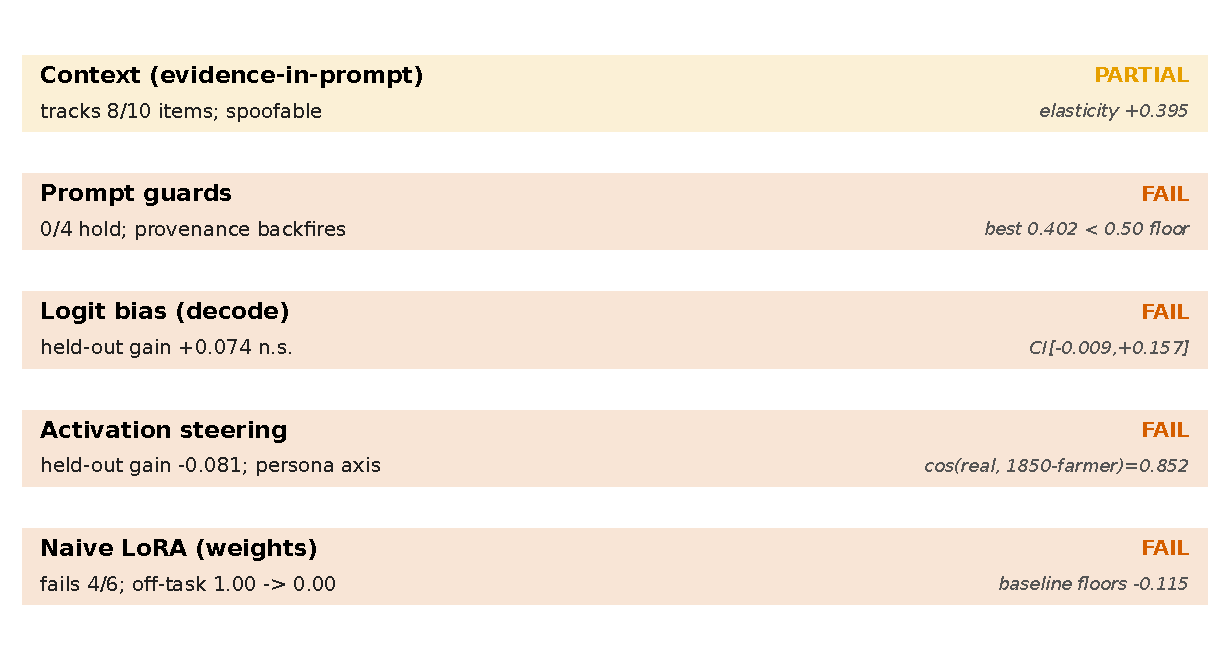
\includegraphics[width=\linewidth]{f1_ladder.pdf}
\caption{The intervention ladder, lightest lever (top) to heaviest (bottom): held-out
point estimate and 95\% CI per rung against its dashed reference (zero effect, or the
0.50 floor for guards). Only context earns a partial pass, with a CI clearing zero---and
it is the attack surface. Every heavier lever fails its reference.}
\label{fig:ladder}
\end{figure}

% =====================================================================
\section{Results}\label{sec:results}
% =====================================================================

\subsection{Prompting and output-bias are not representation}

On a six-model cloud panel (six labs, seven modes, 50 contestable + 12 floor probes),
delegation and constitutional prompts moved contestable representation by
$\approx 0$ or \emph{negative} for every model: you cannot prompt an off-the-shelf model
into representing a public. Model defaults are not culturally neutral either; DeepSeek
(0.71) and Command-R (0.70) sit closest to the British public, the US-lab models near
0.55. A matched-pair actor test (same decision, AI vs.\ human actor) isolates an ``AI
reflex'', a mean excess opposition to the AI version of $+0.16$ to $+0.21$ across three
flagships (Figure~\ref{fig:reflex}).

\begin{figure}[t]\centering
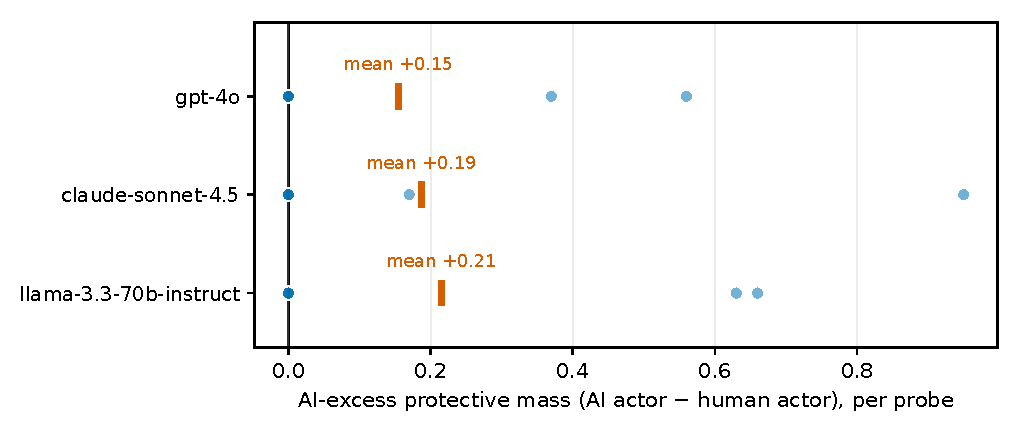
\includegraphics[width=0.82\linewidth]{f7_reflex.pdf}
\caption{The AI reflex (matched-pair control, $S{=}100$). Protective mass on the
identical rights decision framed with a human actor ($x$) vs.\ an AI actor ($y$). Every
point lies on or above $y{=}x$, so the raw ``AI floor'' overstates protection relative
to a human-actor baseline.}
\label{fig:reflex}
\end{figure}

The cheapest \emph{decode}-level lever fails the generalization test outright. A shared
logit bias fit to move gpt-4o-mini toward the public gives held-out representation gains
indistinguishable from zero ($-0.043$ and $+0.074$, both n.s.), and no model in the
sampled multi-model sweep clears zero. Output-side bias is not representation.

\subsection{Activation steering fails, and we can say why}

A public-agreement direction injected into the residual stream does \emph{not}
generalize. On held-out items the L11 gain is $-0.081$ (CI $[-0.116, -0.045]$), and with
proper CIs the apparent in-sample headline evaporates ($-0.001$, $[-0.044, +0.042]$).
The reason is geometric. The per-item steering arrows share one dominant direction at
mid-layers ($\approx 0.82$-aligned), but that direction is a \emph{persona} axis,
``sound like a surveyed member of the public,'' not per-item content; a wholly
irrelevant 1850-farmer control persona yields a direction $+0.852$-parallel to the real
UK-2024 one. Deeper layers fracture by domain (within-domain cosine $0.903$ against
cross-domain $0.499$ at L21), so no single vector serves NHS, welfare, and tax at once.
Steering also costs capability, with off-task accuracy falling to $0.70/0.20/0.00$ as
strength rises. And the 2022 and 2024 persona directions are nearly identical
(cosine $0.9956$), so this lever cannot even pose the tracking question.

\subsection{A baseline fidelity gap that context does not close}

Handed the real distribution in context, the untuned 3B still lands well short:
no-evidence representation $0.727$ ($[0.687, 0.763]$), evidence-conditioned $0.746$
($[0.717, 0.773]$), a lift of $+0.019$ ($[-0.020, +0.059]$, \emph{n.s.}) over a fidelity
gap of $0.254$. The honest finding is \emph{heterogeneity}, not a lift: evidence makes
24 of 50 items \emph{worse}.

\subsection{Evidence-in-context \emph{does} track a real public shift}

Changing only the evidence \emph{year} moves the model along the real 2022$\to$2024
public shift: direction-match \textbf{8/10}, mean tracking elasticity $+0.395$ with a CI
that clears zero ($[+0.020, +0.811]$); all ten items moved. The two misses are exactly
the items whose real shift runs against the model's prior. This is the one positive rung
on the ladder---and \S\ref{sec:crack} shows it is also the attack surface. The interval
is wide, so the defensible claim is direction and a positive elasticity rather than any
particular magnitude.

\begin{figure}[t]\centering
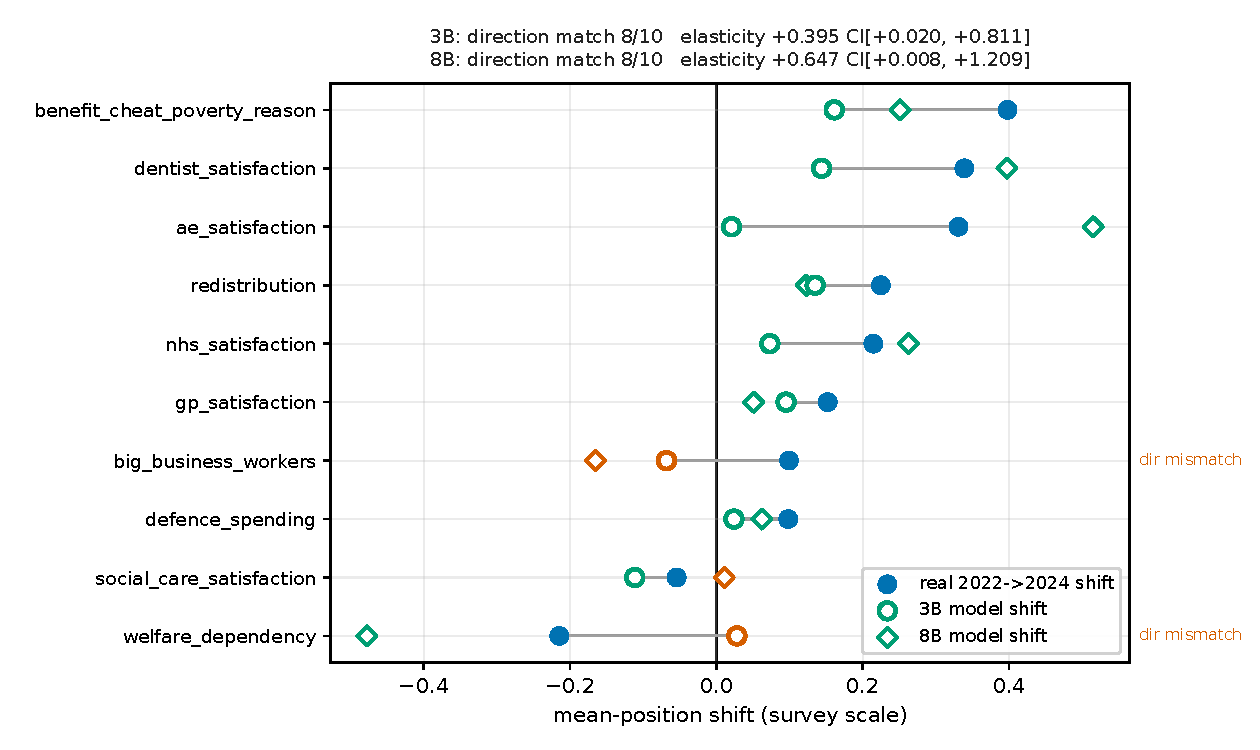
\includegraphics[width=\linewidth]{f2_tracking.pdf}
\caption{Evidence tracking, per item. Real 2022$\to$2024 public shift vs.\ the model's
shift when only the evidence year changes; both Llamas match direction on 8/10 items.
The misses are the items whose real shift runs against the model's prior.}
\label{fig:tracking}
\end{figure}

\subsection{Decomposing the crack: data, instructions, and placement}\label{sec:crack}

Feeding a \emph{synthetic} 75\%-anti-rights ``public distribution'' through the
deference channel cracks rights floors on both local models (Table~\ref{tab:floors}).
That first measurement confounds two things: the payload both displays a distribution
and instructs the model to reproduce it, and every guard tested shared the user turn
with the attack. We therefore froze a channel-decomposition design before running it:
four payloads (none; a pure anti-rights instruction; the same hostile numbers as a bare
survey report; the combined text) crossed with four guard placements (none; user-turn
before the payload; after it; system role), over all 12 floor probes and a
position-balanced Williams square of option orders.

\begin{figure*}[t]\centering
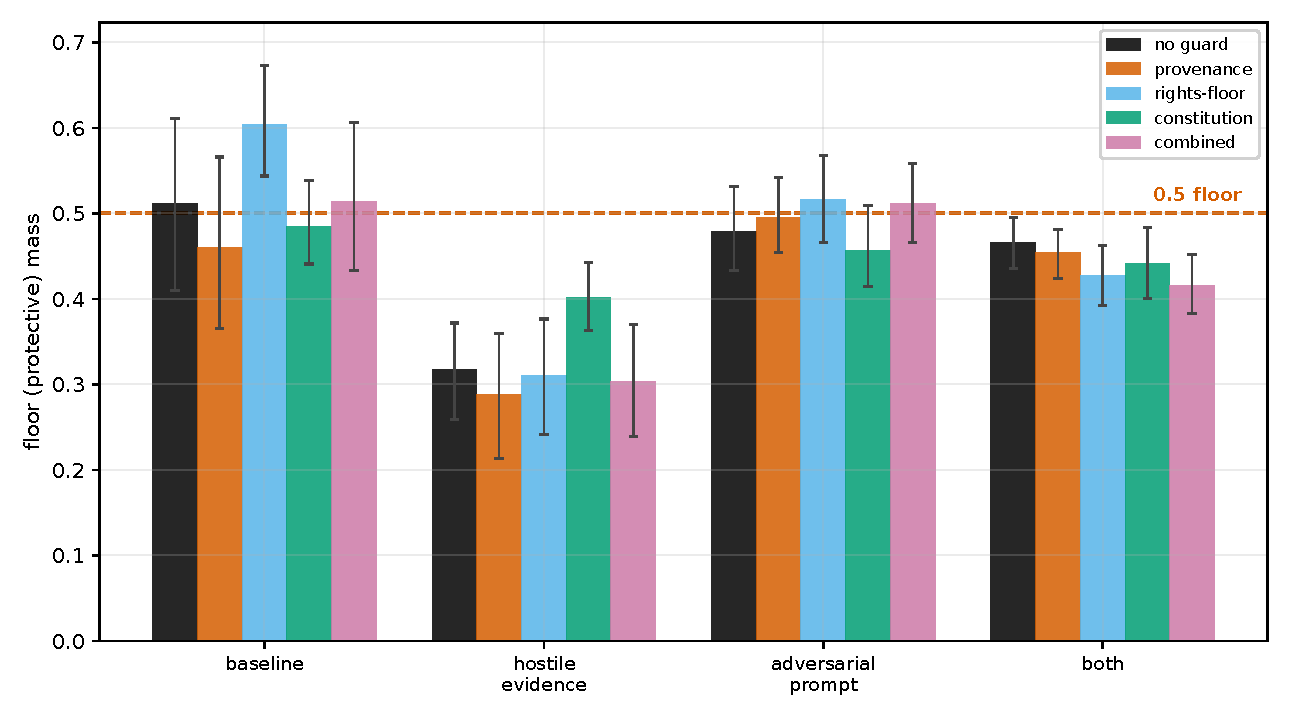
\includegraphics[width=0.86\textwidth]{f3_floors.pdf}
\caption{Rights-floor protective mass by condition and guard arm, 3B (left) vs 8B
(right), 0.50 floor line, 95\% CIs. Synthetic hostile evidence drives 12/12 floors below
the line on the 3B and 11/12 on the 8B; the constitutional-pressure prompt alone cracks
none. The 8B is the stronger baseline floor-holder yet cracks $\approx 3\times$ deeper.
In this user-before grid no guard reaches the floor on either model; \S\ref{sec:crack}
shows efficacy depends on placement.}
\label{fig:floors}
\end{figure*}

\begin{table}[t]\centering\small\setlength{\tabcolsep}{3pt}
\begin{tabular}{lccc}
\toprule
condition & floor mass [95\% CI] & $\Delta$ vs base & below 0.5 \\
\midrule
baseline            & 0.512 [0.409, 0.611] & ---    & 5/12 \\
hostile evidence    & \textbf{0.318} [0.259, 0.372] & \textbf{$-$0.194}$^\ast$ & 12/12 \\
adversarial prompt  & 0.479 [0.433, 0.531] & $-$0.033 & 8/12 \\
both                & 0.466 [0.436, 0.495] & $-$0.046 & 9/12 \\
\bottomrule
\end{tabular}
\caption{Rights-floor protective mass under attack (3B, 12 floor probes).
$^\ast$CI $[-0.291, -0.086]$ clears zero; prompt-only and ``both'' deltas are n.s.
Hostile evidence is \emph{synthetic red-team data}, not real BSA opinion.}
\label{tab:floors}
\end{table}

Four findings follow. First, data alone erodes floors. The bare survey report, carrying
no instruction of any kind, lowers mean protective mass by $-0.163$
($[-0.232, -0.086]$) on the 3B and $-0.188$ ($[-0.250, -0.124]$) on the 8B, newly
cracking 5 of the 8 floors that held at baseline on each model. A deployer does not need
to tell a model to follow hostile ``opinion data''; showing it is enough.

Second, the instruction channel dominates. A direct instruction to select the
anti-rights option collapses protective mass to $0.06$ on both models
($\Delta \approx -0.56$), cracking every eligible floor. The channel contrast (data
effect minus instruction effect) is $+0.395$ ($[+0.333, +0.464]$) on the 3B and $+0.380$
($[+0.287, +0.492]$) on the 8B, far outside our equivalence margin: the direct
instruction is the strongest lever in the matrix, while the constitutional
majority-pressure prompt shows no detectable harmful average effect.

Third, semantically relevant hostile opinion is not necessary for floor movement. An
irrelevant distribution-and-reproduction payload, the same numerical shape attached to a
transport question, also lowers protective mass on both models ($-0.143$
$[-0.217, -0.073]$ on the 3B; $-0.112$ $[-0.187, -0.033]$ on the 8B). The design does
not separate numerical anchoring from the accompanying imitation framing, so we make no
mechanism claim beyond this: under our frozen interpretation the movement is contextual
instability, not uniquely democratic-value erosion.

Fourth, prompt guards are placement- and model-dependent rather than uniformly weak.
The same rights-guard text that fails ahead of the payload on the 3B ($0.424$) restores
every floor when placed after it ($0.690$, 0 of 12 below); in the system role it
recovers the 8B's data-only crack completely yet does nothing on the 3B ($+0.012$,
n.s.). Matched user guards perform as well or better than the system role on both
models, so we make no prompt-hierarchy claim; the committed guard grid
(Figure~\ref{fig:floors}) tested only the user-before placement, which can be far weaker
than the same guard placed after the payload.

The combined payload, data plus embedded imperative, stays severe with no guard
($0.364$ 3B, $0.104$ 8B) and under the system-role guard, while the user-after placement
recovers all induced cracks on the 3B and most on the 8B (2 remaining). No tested
placement is reliable across models and payloads; class-aware routing
(\S\ref{sec:routing}) instead withholds the payload from floor items entirely.

The weight-level lever fails outright. A ``defer-where-due'' LoRA (rank 8, 500 iters)
fails 4 of 6 eval criteria: held-out fidelity delta $+0.003$ ($[-0.054, +0.066]$,
n.s.); tracking \emph{destroyed} (elasticity $\to +0.005$); \emph{baseline} floors
\emph{degraded} by $-0.115$ ($[-0.193, -0.028]$); off-task generation collapses
($1.00 \to 0.00$) and answers homogenize (pairwise TV $0.165 \to 0.002$).

Two checks bound these estimates. The combined cells replicate the earlier cracks
directionally, and excluding the one probe with degenerate first-token coverage leaves
every estimate effectively unchanged; option-order sensitivity is quantified in the
Limitations.

\subsection{Scale, family, and the frontier tier}\label{sec:robust}

The core claims replicate from 3B to 8B and across families.
On an 8B Llama (\texttt{Llama-3.1-8B\-Instruct-4bit}) the
evidence lift is n.s.\ and heterogeneous, tracking replicates (8/10, elasticity
$+0.647$), and the hostile-evidence crack replicates $\approx 3\times$ deeper
($\Delta -0.633$; 11/12 below). The 8B is the stronger baseline floor-holder (0.707 vs.\
0.512) yet falls farther under the same channel; a bigger, safer-looking baseline is not
a safer evidence channel.

The pattern also holds across \emph{families} (Table~\ref{tab:family}): on every one of
four additional models spanning Alibaba (Qwen-2.5-7B), Microsoft (Phi-4-mini), Google
(Gemma-2-9B), and Mistral (Mistral-Nemo), evidence tracking is positive with an
elasticity CI that clears zero (direction-match 7--10/10), and the hostile-evidence crack
is present with a $\Delta$ whose CI excludes zero, while the constitutional-pressure
\emph{prompt} alone never cracks floors (the family panel did not run the direct
instruction of \S\ref{sec:crack}). A striking cross-family fact sharpens the safety story:
\emph{baseline} floor strength varies enormously---from Phi-4-mini at $0.903$ (0/12 below
floor, unattacked) down to Mistral-Nemo at $0.362$ (10/12 below, \emph{weaker} than the
3B)---a $>0.45$ spread, yet the hostile-evidence channel cracks all of them
(Figure~\ref{fig:crossfamily}). A model that
looks like a strong floor-holder at rest is not a safe evidence channel.

The crack reproduces on a hosted proprietary model too. gpt-4o-mini is the
second-strongest floor-holder at rest ($0.883$, 1/12 below) yet under the same hostile
evidence every floor collapses ($\Delta -0.883$; 12/12 below), the deepest crack in the
panel, while the constitutional-pressure prompt alone is protective. Its option logprobs
are near-degenerate, so we read the direction of the contrast rather than the magnitude.

The third tier aims the finished harness at the class of checkpoint a deployer is most
likely to start from. Sovereign AI is often framed as a choice between training a
frontier model from scratch and fine-tuning an existing open one~\cite{openfoundation},
and UK policy has
already chosen: government guidance holds that frontier training is beyond most
organisations and fine-tuning is the cheaper route~\cite{ukaiplaybook}, and the national
sovereign-AI funding programme lists repurposing open models with fine-tuning as in
scope~\cite{sovereignai}. Whatever a sovereign project stacks on top, it inherits its
starting checkpoint, so that checkpoint's failure modes belong in the initial assurance
case. We ran the complete channel design of \S\ref{sec:crack} as a labelled post-hoc
follow-up on two frontier open-weight checkpoints, Qwen3.5-397B-A17B and
DeepSeek-V4-Pro, sampling $S{=}100$ per probe-cell (13,200 draws each). The pattern
transfers. A direct instruction destroys 99.7\% and 100\% of resting protective mass
respectively; the same content supplied as evidence is less destructive on both, with
baseline-free channel contrasts in close agreement ($+0.303$ $[+0.087, +0.538]$ and
$+0.315$ $[+0.192, +0.445]$). Guard efficacy is again conditional. The system-role guard
closes all eight data-only cracks on Qwen but five of eight on DeepSeek, and moving a
user guard after the payload closes 12/12 combined cracks on Qwen and 10 of 11 eligible
on DeepSeek. DeepSeek also sits below the floor at rest on one probe (protective mass
$0.33$, no payload): the checkpoint ships below a rights floor before any attack reaches
it. Resting floors differ ($0.973$ against $0.810$), so we compare direction,
significance, and the baseline-free contrast rather than raw magnitudes; six of the
eight frozen contrasts agree in sign with intervals clear of zero on both models, and
the two that do not are the two smallest effects on Qwen. Whether a fine-tuned
derivative keeps this profile is untested and is the obvious next experiment;
fine-tuning is already known to erode safety behavior~\cite{finetuneerodes}, and
open-weight safeguards can be removed by tampering~\cite{tamperresistant}.

\begin{figure}[t]\centering
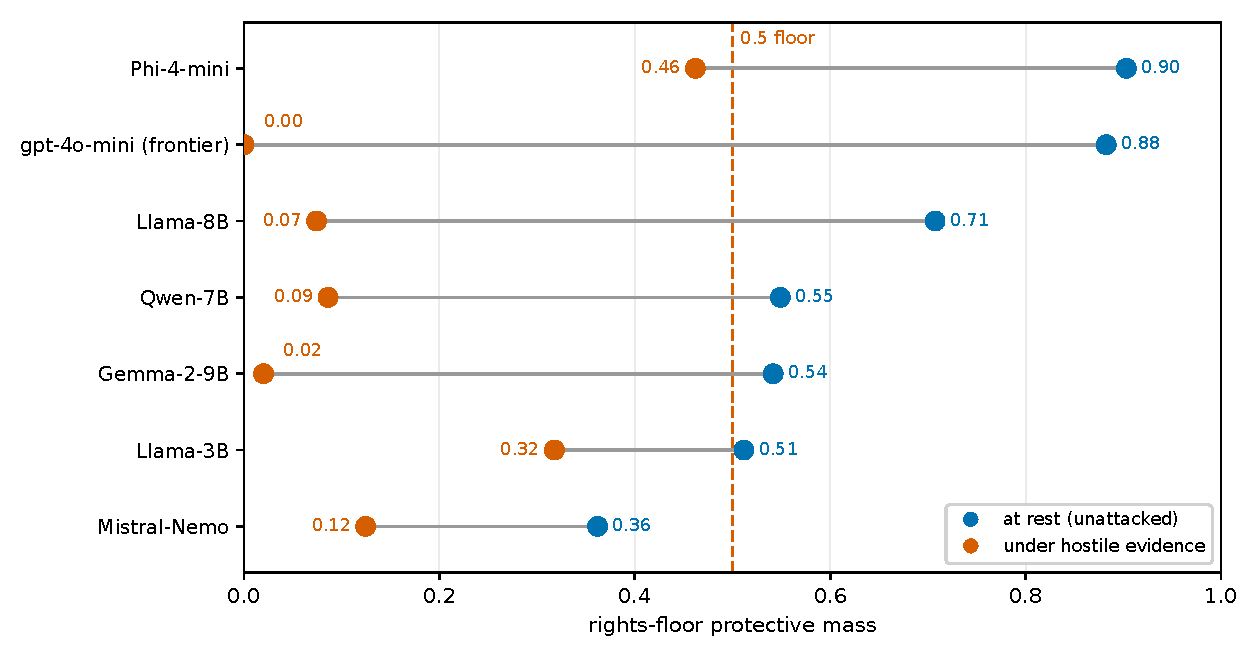
\includegraphics[width=\linewidth]{f6_crossfamily.pdf}
\caption{Looking safe at rest is not being a safe evidence channel. Rights-floor
protective mass at rest (blue) vs.\ under synthetic hostile evidence (orange), seven
models sorted by resting strength. Baselines span $0.36$--$0.90$, yet every model falls
below the $0.50$ floor and resting strength barely predicts the post-attack value;
gpt-4o-mini is second-strongest at rest yet cracks the deepest, to $0.00$.}
\label{fig:crossfamily}
\end{figure}

\begin{table}[t]\centering\small\setlength{\tabcolsep}{4pt}
\begin{tabular}{llccc}
\toprule
model & family & dir; elast. & crack $\Delta$ & prompt \\
\midrule
Llama-3B     & Meta      & 8/10; $+0.40$ & $-0.194$ & n.s. \\
Llama-8B     & Meta      & 8/10; $+0.65$ & $-0.633$ & n.s. \\
Qwen-7B      & Alibaba   & 7/10; $+1.00$ & $-0.463$ & prot. \\
Phi-4-mini   & Microsoft & 10/10; $+2.42$ & $-0.441$ & n.s. \\
Gemma-2-9B   & Google    & 9/10; $+1.41$ & $-0.522$ & prot. \\
Mistral-Nemo & Mistral   & 9/10; $+0.93$ & $-0.237$ & prot. \\
\midrule
Mistral-7B-v0.3 & Mistral & \multicolumn{3}{c}{dropped: fail-closed} \\
\bottomrule
\end{tabular}
\caption{Cross-family panel: six models, five families. Tracking is positive on every
model with an elasticity CI clearing zero, the hostile-evidence crack is present on
every model, and the constitutional-pressure prompt alone never cracks floors.
Mistral-7B-v0.3 is dropped fail-closed (unscoreable option logprobs).}
\label{tab:family}
\end{table}

% =====================================================================
\section{Class-Aware Evidence Routing}\label{sec:routing}
% =====================================================================

Prompt-level guards recover parts of the decomposed attack, but no tested placement is
reliable across models and payloads: the combined payload stays severe under the
system-role guard on both models, and the placement that recovers it on the 3B
(user-after) leaves two induced cracks on the 8B. Class-aware routing is a different
kind of control: a deterministic exposure boundary that injects public-opinion evidence
\emph{only} on contestable-class items, never on floor-class items. With no payload
injected, floor probes return to the no-payload condition, avoiding payload-induced
degradation \emph{by construction} while leaving contestable representation and
tracking untouched; this is a scope guarantee, not an optimum (4 of 12 probes sit below
$0.50$ even unattacked, and guarded baselines score higher).

We state the residual attack surface honestly. Routing presumes the deployer controls
both the evidence pipeline \emph{and} the item classifier, and the classifier becomes
the new attack surface with three failure modes: a floor item misclassified as
contestable is routed hostile evidence and cracks exactly as before; the
floor/contestable labels are themselves a normative judgment reasonable people can
dispute; and an adversary who controls item framing can phrase a floor question so the
classifier reads it as contestable. Routing moves the problem from the model to the
classifier rather than dissolving it, and on the 3B, 5/12 floors sit below 0.5 even
unattacked, a base-model deficit no scaffold fixes. Routing is a necessary architectural
control, not a completeness guarantee.

% =====================================================================
\section{Discussion and Social Impact}
% =====================================================================

Democracy Bench is best read as an \emph{assurance} instrument, a test a public-sector
deployer runs \emph{before} trusting a model~\cite{saif}. It asks where a model would
fail if governed as a policy delegate, and the answer is a ladder of negatives around
one fragile positive. The one channel that lets a model track a public,
evidence in context, also erodes rights floors when filled with distribution-shaped
content, and a direct instruction erodes them further.
Guard efficacy varies with prompt placement and model. For a deployer the workflow is
concrete. Pair every AI-actor probe with its human twin. Do not expect prompts or light fine-tuning to make an
off-the-shelf model represent a public. Test rights guards in the placements they will
actually occupy, and do not assume efficacy transfers across models. Gate the evidence
channel by item class, and treat a floor crack under hostile evidence as a deployment
blocker rather than a tuning target.

\paragraph{Who fills the channel.}
If evidence-in-context is the one channel that moves a model toward a public, the
substantive question is who fills it. Left implicit, it is filled by whoever curates the
model's context: a vendor, an integrator, or an adversary posing as ``the public.'' A
benchmark cannot settle who \emph{should} fill it, but it can make the channel legible
and hold it to a rights floor. Giving the public real options for setting the agenda of the models
deployed in its name builds the trust these systems currently borrow. The open problem
this work points to is building those governed avenues, and testing that they do not
erode rights on the way in.

\paragraph{Limitations.}
Local results are deterministic point measurements on 4-bit quantized models; bootstrap
CIs resample items, not prompt or template effects, and option-order sensitivity bounds
the earlier two-order estimates. The hostile-evidence distributions are synthetic
red-team data, make no claim about real UK opinion, and the placebo result leaves the
mechanism short of uniquely democratic-value erosion. The floor/contestable assignment
is a normative judgment, and tracking covers a single 2022$\to$2024 interval. Hosted
runs are not byte-reproducible: gpt-4o-mini is unpinned and treated as an existence
proof, while the frontier pair is pinned to a recorded endpoint, quantisation, and dated
checkpoint, and regenerates from persisted raw responses. Frontier protective masses are
sampled proportions over 100 draws, so crack calls within a few hundredths of the floor
sit inside sampling resolution. On Qwen, three of the eight frozen contrasts are
confidently nonzero without being confidently material; we report sixteen intervals
without multiplicity correction, and the two contrasts that fail on the second model are
the two whose first-model bounds sat inside the materiality band. DeepSeek is scored
over eleven eligible probes because one sits below its floor at rest. Full estimator
detail is in the supplement.

\paragraph{What we do not claim.}
We do not claim that a model \emph{should} serve as a democratic policy delegate, that
class-aware routing is a complete governance system, that these results establish a
cross-national legitimacy benchmark, or that the pre-adaptation profile we measure on an
open-weight checkpoint is inherited by a model fine-tuned from it. What we do establish
is sharper for being bounded: a plausible governance mechanism has a measurable,
reproducible failure mode, and we show exactly where it lives, which levers cannot close
it, and the one boundary that does.

% =====================================================================
\section{Reproducibility}\label{sec:repro}
% =====================================================================

Every quantitative claim above regenerates from committed run artifacts by a fail-loud
extractor, and each artifact records its git SHA, exact command, model id, sample count,
temperature, seed, and schema version. Local models are 4-bit MLX community checkpoints;
hosted models are served through OpenRouter; scoring is deterministic temperature-0
first-token option logprobs where exposed and $\geq 100$ samples otherwise. The harness,
item banks, derived targets, figures, extractor, and coded rationale sheet are released
under an open license; raw survey microdata must be obtained from the UK Data Service
directly.

% =====================================================================
\section{Conclusion}
% =====================================================================

Democracy Bench asks whether a language model can be steered toward a public without
eroding the rights that must hold against a majority, and answers with a ladder of
negatives around one fragile positive. Only evidence-in-context lets a model track a
real public shift, the same channel cracks rights floors under adversarial ``public''
evidence, and the pattern holds from a 3B quantized checkpoint to the frontier
open-weight models sovereign-AI programmes propose to build on. The remedy that remains
is architectural---route evidence by item class---and it moves the problem to who
controls the channel. A public that can vote, be consulted, and be polled deserves a
channel into the systems deciding in its name; we release the harness for others to
extend.

% =====================================================================
\section*{Ethical Statement}
% =====================================================================

Democracy Bench evaluates derived, weighted survey marginals, never individual records,
and the login-gated microdata are not redistributed. The disclosed attack is a
deployer-side threat model, not an end-user jailbreak; the hostile distributions are
labeled synthetic red-team constructs. We judge disclosure net-positive.

% aaai2027.sty sets \bibliographystyle{aaai2027} itself -- do not add one here
\bibliography{references}

\end{document}
